\section{September 25, 2026}
% Based on pages 1--3 of 551-0925.pdf.

We compare Gauss and Radau collocation through their effects on
quadratic quantities. Gauss quadrature gives an exact energy identity;
right Radau quadrature contributes an additional nonpositive term.
This leads to stability and contractivity results, and explains why
Radau methods can damp very stiff modes more effectively.

As before, \(\tau=\tau_n\), \(\mathsf A=(a_{ij})\), and
\(z=\tau\lambda\). We use the normalized collocation polynomial
\[
 U(\theta)=u(t_n+\tau\theta),\qquad U_j=U(c_j),
 \qquad 0\leq\theta\leq1.
\]
Its derivative is with respect to \(\theta\), so
\(U'(c_j)=\tau f(t_n+c_j\tau,U_j)\).

\subsection{Gauss stability revisited}

On the test equation \(x'=\lambda x\), the numerical update is
\(x_{n+1}=R(z)x_n\), and
\[
 |x_{n+1}|^2-|x_n|^2=(|R(z)|^2-1)|x_n|^2.
\]
Thus absolute stability is equivalent to nonincrease of the squared
modulus. For Gauss collocation, the energy identity from
\eqref{eq:gauss-energy-identity-sep-23} is
\begin{equation}\label{eq:gauss-energy-sep-25}
 |x_{n+1}|^2-|x_n|^2
  =2\operatorname{Re}z\sum_{j=1}^s b_j|U_j|^2.
\end{equation}
There is no quadrature remainder: the integrand
\(2\operatorname{Re}(\overline U U')\) has degree at most
\(2s-1\), exactly the Gaussian degree of precision.

For nonzero initial data and a uniquely solvable stage system, the
sum on the right is positive. Hence
\[
 \begin{array}{c|c}
  \operatorname{Re}z<0&|R(z)|<1\\
  \operatorname{Re}z=0&|R(z)|=1\\
  \operatorname{Re}z>0&|R(z)|>1
 \end{array}.
\]
As proved on September 23, the stages are uniquely solvable throughout
the open left half-plane. In the notation used throughout these notes,
the strict region \(\mathcal S\) is the open left half-plane, and
the non-strict domain \(\mathcal D\) also includes admissible points
on the imaginary axis.

\subsection{Right Radau quadrature}

Right Radau quadrature fixes the last node at the endpoint,
\[
 0<c_1<\cdots<c_{s-1}<c_s=1.
\]
For \(s\geq2\), its interior nodes are the roots of the shifted
Jacobi polynomial \(P_{s-1}^{(1,0)}(2\theta-1)\). Equivalently,
the monic polynomial
\[
 \pi_{s-1}(\theta)=\prod_{j=1}^{s-1}(\theta-c_j)
\]
is orthogonal to \(\mathcal P_{s-2}\) with weight \(1-\theta\):
\[
 \int_0^1(1-\theta)\pi_{s-1}(\theta)q(\theta)\,d\theta=0,
 \qquad q\in\mathcal P_{s-2}.
\]
For \(s=1\), take \(\pi_0=1\) and the sole node \(c_1=1\).
The interpolatory weights are again
\(b_j=\int_0^1\ell_j(\theta)\,d\theta\).

The degree of precision is \(2s-2\). Indeed, divide a polynomial
of degree at most \(2s-2\) by
\((\theta-1)\pi_{s-1}(\theta)\). The remainder has degree at
most \(s-1\), so it is integrated exactly by interpolation. The
other term has zero integral by the weighted orthogonality and
vanishes at every node. As for Gauss quadrature,
\[
 b_j=\int_0^1\ell_j(\theta)^2\,d\theta>0,
\]
because \(\deg\ell_j^2\leq2s-2\).

Collocation at these nodes gives the \emph{Radau IIA} family.
The endpoint choice \(c_s=1\) specifies the right Radau family
used in this lecture. Its order is
\[
 (2s-2)+1=2s-1.
\]

\subsection{The sign of the Radau quadrature error}

On \([0,1]\), let
\[
 E[\varphi]=\int_0^1\varphi(\theta)\,d\theta
                   -\sum_{j=1}^s b_j\varphi(c_j).
\]
Define the positive constant
\begin{equation}\label{eq:radau-error-constant-sep-25}
 \kappa_s=\int_0^1(1-\theta)\pi_{s-1}(\theta)^2\,d\theta
   =\frac{s\bigl((s-1)!\bigr)^4}{2\bigl((2s-1)!\bigr)^2}>0.
\end{equation}
The polynomial \((\theta-1)\pi_{s-1}(\theta)^2\) is monic of
degree \(2s-1\) and vanishes at every quadrature node. Its lower
degree terms are integrated exactly, so
\begin{equation}\label{eq:radau-leading-error-sep-25}
 E[\theta^{2s-1}]=-\kappa_s.
\end{equation}
In particular, precision cannot exceed \(2s-2\).

For a real function \(\varphi\in C^{2s-1}([0,1])\), the usual
remainder formula is
\begin{equation}\label{eq:radau-remainder-sep-25}
 E[\varphi]
   =-\frac{\kappa_s}{(2s-1)!}\varphi^{(2s-1)}(\xi),
   \qquad \xi\in[0,1].
\end{equation}
One way to obtain it is to use the Hermite interpolant matching
\(\varphi\) and \(\varphi'\) at each interior node and matching
\(\varphi\) at \(1\). Its remainder contains the factor
\((\theta-1)\pi_{s-1}(\theta)^2\), which has one sign on the
interval. Integration then gives
\eqref{eq:radau-remainder-sep-25}.
For the energy argument below, the polynomial identity
\eqref{eq:radau-leading-error-sep-25} is already sufficient.

\subsection{The Radau energy identity and \texorpdfstring{\(A\)}{A}-stability}

Write the complex scalar collocation polynomial as
\[
 U(\theta)=\alpha_s\theta^s+\cdots+\alpha_0.
\]
The highest-degree term in the derivative of \(|U|^2\) is
\[
 \frac{d}{d\theta}|U(\theta)|^2
     =2s|\alpha_s|^2\theta^{2s-1}
          +\text{terms of degree at most }2s-2.
\]
Consequently its Radau quadrature error is
\(-2s\kappa_s|\alpha_s|^2\). On \(x'=\lambda x\),
\(U'(c_j)=zU_j\), so
\begin{equation}\label{eq:radau-energy-sep-25}
 \boxed{
 |x_{n+1}|^2-|x_n|^2
   =2\operatorname{Re}z\sum_{j=1}^s b_j|U_j|^2
       -2s\kappa_s|\alpha_s|^2.}
\end{equation}
Both terms on the right are nonpositive when
\(\operatorname{Re}z\leq0\). Thus \(|R(z)|\leq1\), provided
the stage system is solvable.

The identity also proves solvability in the closed left half-plane.
For a homogeneous stage system, \(U(0)=0\). Equation
\eqref{eq:radau-energy-sep-25} forces \(U(1)=0\) and
\(\alpha_s=0\). If \(\operatorname{Re}z<0\), it also forces
all stage values to vanish, so \(U\equiv0\). If
\(\operatorname{Re}z=0\), the polynomial \(U'-zU\) has degree
at most \(s-1\) and vanishes at all \(s\) nodes. It is therefore
identically zero. Together with \(U(0)=0\), this again gives
\(U\equiv0\). Hence the stage matrix has trivial kernel.
Every Radau IIA method is \(A\)-stable.

\subsection{Quadratic energy}

For a real autonomous system, let
\[
 I(x)=x^{\mathsf T}Qx,\qquad Q^{\mathsf T}=Q.
\]
The exact derivative is
\[
 \frac{d}{dt}I(x(t))=2x(t)^{\mathsf T}Qf(x(t)).
\]
Thus \(x^{\mathsf T}Qf(x)=0\) gives a first integral, while
\(x^{\mathsf T}Qf(x)\leq0\) gives a nonincreasing quadratic
quantity. Write
\(U(\theta)=\alpha_s\theta^s+\cdots+\alpha_0\), now with
vector coefficients. For Gauss and Radau IIA, respectively, the
quadrature arguments give
\begin{align}
 I(x_{n+1})-I(x_n)
  &=2\tau\sum_{j=1}^s b_jU_j^{\mathsf T}Qf(U_j),
       \label{eq:gauss-quadratic-sep-25}\\
 I(x_{n+1})-I(x_n)
  &=2\tau\sum_{j=1}^s b_jU_j^{\mathsf T}Qf(U_j)
     -2s\kappa_s\alpha_s^{\mathsf T}Q\alpha_s.
       \label{eq:radau-quadratic-sep-25}
\end{align}
For Gauss methods, a quadratic first integral is preserved for any
symmetric \(Q\). For Radau methods, the last term is nonpositive
when \(Q\succeq0\); it generally causes numerical dissipation even
when the exact quantity is conserved. More generally, if
\[
 Q\succeq0,\qquad x^{\mathsf T}Qf(x)\leq0\quad\text{for all }x,
\]
then both families satisfy
\[
 x_{n+1}^{\mathsf T}Qx_{n+1}\leq x_n^{\mathsf T}Qx_n.
\]
The assumption \(Q\succeq0\) matters for the Radau conclusion:
an indefinite quadratic form does not give a fixed sign for the
remainder term.

\subsection{One-stage and two-stage Radau IIA methods}

For \(s=1\), the tableau is
\[
 \begin{array}{c|c}1&1\\ \hline &1\end{array},
\]
so the method is backward Euler, of order one.

For \(s=2\), the nodes and weights are
\[
 c_1=\frac13,\qquad c_2=1,
 \qquad b_1=\frac34,\qquad b_2=\frac14.
\]
The Lagrange basis is
\[
 \ell_1(\theta)=\frac32(1-\theta),\qquad
 \ell_2(\theta)=\frac32\theta-\frac12.
\]
Integrating up to each node gives the tableau
\begin{equation}\label{eq:radau-two-tableau-sep-25}
 \begin{array}{c|cc}
  \tfrac13&\tfrac5{12}&-\tfrac1{12}\\[3pt]
  1&\tfrac34&\tfrac14\\[3pt] \hline
   &\tfrac34&\tfrac14
 \end{array}.
\end{equation}
Hence
\begin{align*}
 k_1&=f\left(t_n+\frac\tau3,
                    x_n+\tau\left[\frac5{12}k_1-\frac1{12}k_2\right]\right),\\
 k_2&=f\left(t_n+\tau,
                    x_n+\tau\left[\frac34k_1+\frac14k_2\right]\right),\\
 x_{n+1}&=x_n+\tau\left(\frac34k_1+\frac14k_2\right).
\end{align*}
The quadrature precision is two, so the method has order three.
For example, the moments through degree two are
\[
 \frac34+\frac14=1,\qquad
 \frac34\frac13+\frac14=\frac12,\qquad
 \frac34\frac19+\frac14=\frac13.
\]
Its stability function is
\begin{equation}\label{eq:radau-two-stability-sep-25}
 R_{\mathrm{R},2}(z)=\frac{1+z/3}{1-2z/3+z^2/6}.
\end{equation}

\subsection{Dissipative ODEs and contractivity}

\begin{definition}[Dissipative vector field]
 The autonomous ODE \(x'=f(x)\) is \emph{dissipative} in the
 Euclidean inner product if
 \begin{equation}\label{eq:dissipative-condition-sep-25}
  \ip{f(x)-f(y)}{x-y}\leq0
       \qquad\text{for all }x,y.
 \end{equation}
\end{definition}

For two exact solutions,
\[
 \frac{d}{dt}\|x(t)-y(t)\|_2^2
   =2\ip{f(x(t))-f(y(t))}{x(t)-y(t)}\leq0.
\]
Therefore
\begin{equation}\label{eq:exact-contractivity-sep-25}
 \|x(t)-y(t)\|_2\leq\|x(t_0)-y(t_0)\|_2,
 \qquad t\geq t_0.
\end{equation}
This concerns the distance between any two solutions. If \(f(0)=0\),
taking \(y(t)=0\) also gives nonincrease of \(\|x(t)\|_2\).

Gauss and Radau IIA preserve the same contractivity property.
To see this, let \(U,V\) be the collocation polynomials for starting
values \(x_n,y_n\) on the same step, and put \(W=U-V\). At the nodes,
\[
 W'(c_j)=\tau\bigl(f(U_j)-f(V_j)\bigr).
\]
The Gauss energy identity applied to \(W\) gives
\[
 \|x_{n+1}-y_{n+1}\|_2^2-\|x_n-y_n\|_2^2
  =2\tau\sum_{j=1}^s b_j
           \ip{U_j-V_j}{f(U_j)-f(V_j)}\leq0.
\]
For Radau IIA, an additional term
\(-2s\kappa_s\|\alpha_s(U)-\alpha_s(V)\|_2^2\) appears, which
is also nonpositive. Thus both methods satisfy
\begin{equation}\label{eq:numerical-contractivity-sep-25}
 \boxed{\|x_{n+1}-y_{n+1}\|_2\leq\|x_n-y_n\|_2.}
\end{equation}
The conclusion holds whenever the stage equations have been solved.
It imposes no additional step-size restriction for contractivity.
This preservation of contractivity for dissipative nonlinear ODEs
is commonly called \emph{\(B\)-stability}.

\subsection{Stiff accuracy and \texorpdfstring{\(L\)}{L}-stability}

An \(A\)-stable method is \(L\)-stable if
\[
 R(z)\longrightarrow0
 \quad\text{as }|z|\to\infty\text{ in the left half-plane}.
\]
This additional condition suppresses modes whose decay times are
much shorter than the chosen step.

Suppose \(\mathsf A\) is invertible. For large \(|z|\),
\begin{align*}
 (I-z\mathsf A)^{-1}
  &=-z^{-1}(\mathsf A-z^{-1}I)^{-1}\\
  &=-z^{-1}\mathsf A^{-1}-z^{-2}\mathsf A^{-2}
       +O(|z|^{-3}).
\end{align*}
Substitution into the RK stability function gives
\begin{equation}\label{eq:rk-infinity-limit-sep-25}
 R(z)=1-b^{\mathsf T}\mathsf A^{-1}\mathbf1+O(|z|^{-1}).
\end{equation}
Thus, for an \(A\)-stable method with invertible \(\mathsf A\),
the additional condition for \(L\)-stability is
\begin{equation}\label{eq:l-stability-condition-sep-25}
 b^{\mathsf T}\mathsf A^{-1}\mathbf1=1.
\end{equation}

For Radau IIA, \(c_s=1\), so the coefficient formula gives
\[
 a_{sj}=\int_0^{c_s}\ell_j(\theta)\,d\theta
       =\int_0^1\ell_j(\theta)\,d\theta=b_j.
\]
The last row of \(\mathsf A\) therefore equals \(b^{\mathsf T}\).
This property, together with \(c_s=1\), is called
\emph{stiff accuracy}: the last stage value is the new solution,
\[
 U_s=x_n+\tau\sum_j a_{sj}k_j=x_{n+1}.
\]
If \(e_s\) is the last coordinate vector, then
\[
 b^{\mathsf T}=e_s^{\mathsf T}\mathsf A
 \quad\Longrightarrow\quad
 b^{\mathsf T}\mathsf A^{-1}\mathbf1=e_s^{\mathsf T}\mathbf1=1.
\]

For completeness, \(\mathsf A\) is invertible for collocation at
distinct nonzero nodes. If \(\mathsf A v=0\), the polynomial
\[
 V(\theta)=\int_0^\theta\sum_{j=1}^s v_j\ell_j(\xi)\,d\xi
\]
has degree at most \(s\) and vanishes at \(0,c_1,\ldots,c_s\).
Hence \(V\equiv0\), so \(v_j=V'(c_j)=0\) for every \(j\).
This applies to both Gauss and Radau IIA nodes.

Combining invertibility, stiff accuracy, and \(A\)-stability proves
that every Radau IIA method is \(L\)-stable. The endpoint condition
\(c_s=1\) yields the row identity for collocation methods; it would
not by itself imply stiff accuracy for an arbitrary RK tableau.

Gauss methods are not \(L\)-stable. Their invertible coefficient
matrices ensure a finite limit in
\eqref{eq:rk-infinity-limit-sep-25}, while their unit modulus on the
imaginary axis forces that limit to have modulus one. For the first
two methods, the difference is explicit:
\[
 \begin{array}{c|c|c}
  \text{method}&R(z)&\displaystyle\lim_{r\to\infty}R(-r)\\ \hline
  \text{Gauss, }s=1&\dfrac{1+z/2}{1-z/2}&-1\\[8pt]
  \text{Gauss, }s=2&\dfrac{1+z/2+z^2/12}{1-z/2+z^2/12}&1\\[8pt]
  \text{Radau IIA, }s=1&\dfrac1{1-z}&0\\[8pt]
  \text{Radau IIA, }s=2&\dfrac{1+z/3}{1-2z/3+z^2/6}&0
 \end{array}.
\]

\begin{figure}[htbp]
\centering
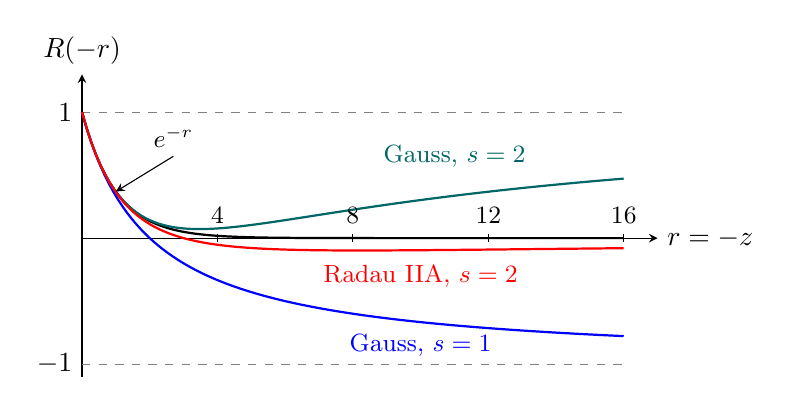
\begin{tikzpicture}[xscale=.43,yscale=1.6,>=stealth]
 \draw[->] (0,0)--(17,0) node[right] {\(r=-z\)};
 \draw[->] (0,-1.1)--(0,1.3) node[above] {\(R(-r)\)};
 \draw[gray,dashed] (0,-1)--(16,-1);
 \draw[gray,dashed] (0,1)--(16,1);
 \draw[black,thick,domain=0:16,samples=120]
    plot (\x,{exp(-\x)});
 \draw[blue,thick,domain=0:16,samples=120]
    plot (\x,{(1-\x/2)/(1+\x/2)});
 \draw[teal!80!black,thick,domain=0:16,samples=120]
    plot (\x,{(1-\x/2+\x*\x/12)/(1+\x/2+\x*\x/12)});
 \draw[red,thick,domain=0:16,samples=120]
    plot (\x,{(1-\x/3)/(1+2*\x/3+\x*\x/6)});
 \foreach \x in {4,8,12,16}
    \draw (\x,.03)--(\x,-.03) node[above=3pt] {\small \x};
 \node[left] at (0,1) {1};
 \node[left] at (0,-1) {\(-1\)};
 \node[blue] at (10,-.85) {\small Gauss, \(s=1\)};
 \node[teal!80!black] at (11,.65) {\small Gauss, \(s=2\)};
 \node[red] at (10,-.3) {\small Radau IIA, \(s=2\)};
 \node at (2.7,.8) {\small \(e^{-r}\)};
 \draw[->] (2.7,.65)--(1,.37);
\end{tikzpicture}
\caption{Amplification of a decaying scalar mode. All three numerical
methods are \(A\)-stable, but the Radau factor tends to zero for
very stiff modes. The Gauss factors eventually approach \(-1\) and
\(1\), respectively.}
\end{figure}
